\section{Zukünftige Arbeit}
Es gibt einige Möglichkeiten den vorgestellten Entwurf
zu verbessern und zu erweitern. Denn um mit modernen SAT-Solvern
mithalten zu können, muss die Anzahl möglicher Variablen
weiter erhöht werden. Auch über eine bessere Kommunikation zwischen
FPGA und Host-PC muss man nachdenken (Abschnitt \ref{kommu}).\\
Ein klarer Schwachpunkt im Entwurf ist der Speicherverbrauch.
So beschränken die Literal-Lookup-Tabellen, durch ihren 
einfachen Aufbau, die Variablenanzahl auf 1024 mögliche Variablen.
Noch viel stärker wird die Variablenanzahl durch die 
Übersetzungstabelle im Literal-Arbiter eingeschränkt (256 Variablen).
Obwohl 2048 Klauseln pro Propagation-Engine
möglich wären, wird auch deren Zahl durch die Übersetzungstabelle
auf 128 Klauseln pro Propagation-Engine begrenzt. Aus der Tatsache,
das der Block-RAM-Speicher knapp ist, folgt außerdem, das maximal 32 Propagation-Engines
erzeugt werden können, was die lösbaren Problemdateien weiter
einschränkt.\\
In der Arbeit von Davis \cite{davis:2008} ist es dem FPGA-SAT-Solver
möglich bis zu $2^{16}$ Variablen und Klauseln bei maximal 64
Gruppen zu verarbeiten. Sie verwenden einen Xilinx Virtex-5 
XC5VLX110T FPGA mit mehr als doppelt soviel Block-RAM (296 x 18Kbit).
Die Literal-Übersetzungstabelle wird komplett in einem
DRAM gespeichert, so dass alle Block-RAMs für die Propagation-Engines
zur Verfügung stehen. Statt einer einfachen Literal-Lookup-Tabelle
benutzt Davis einen Baum im Block-RAM-Speicher, 
um Variablentupel wiederzufinden. Dieser Baum macht es möglich
wesentlich mehr Variablen zu referenzieren. 
Eine weitere Möglichkeit, die Lösungszeit des FPGA-Solvers
zu optimieren, ist es statt des DPLL-Algorithmus den CDCL-Algorithmus zu
nutzen. Welche Möglichkeiten der CDCL-Algorithmus bietet,  
wird in Abschnitt \ref{cdcl} diskutiert.
Wie der Entwurf erweitert werden kann, 
um größere Formeln zu lösen, wird in Abschnitt \ref{bigformula} 
vorgestellt. In Abschnitt \ref{treelookup} wird der bereits
angesprochene baumstruckturierte Literal-Lookup erläutert.

\subsection{Lösen größerer Formeln}
\label{bigformula}
Die lösbare Formelgröße wird primär durch den verfügbaren
Speicher in der Literal-Übersetzungstabelle bestimmt.
Denn eigentlich entspricht der Inhalt der Tabelle der
vollständigen Formel. Jedem Literal wird darin seine
Gruppe, Klausel und Position zugewiesen, was einer
eindeutigen Positionsbestimmung innerhalb der Formel
gleichkommt. Je mehr Speicher in der 
Literal-Übersetzungstabelle zur Verfügung steht, um so
größere Formeln können gelöst werden. Im 
vorgestellten Entwurf steht dieser Tabelle
nur ein Teil des Block-RAMs des FPGAs zur Verfügung, so
dass nur kleine Formeln lösbar sind. Auf dem
genutzten ML505-Board exisitiert jedoch ein 9 Mbit
großer SRAM-Speicher (256k x 36 Bit). Es besteht
die Möglichkeit die Übersetzungstabelle in den 
vorhandenen SRAM-Speicher auszulagern.
So könnte man 64 Gruppen (6 Bit), 1024 Klauseln
(10 Bit) pro Gruppe und 8 Literale (3 Bit) pro 
Klausel realisieren. Mit 17 Bit pro Literal
ergibt sich ein ein Gesamtspeicherbedarf
von ca. 8,9 Mbit ($2^{19}$ x 17 Bit). Die 8,9 Mbit große 
Übersetzungstabelle passt vollständig in den 
SRAM-Speicher des Entwicklerboards.\\
Desweiteren wird die Problemgröße durch
die Literal-Lookup-Tabellen in den
Propagation-Engines bestimmt. Eine
Literal-Lookup-Tabelle kann maximal
auf 1024 Variablentupel zeigen, was
bedeutet, dass die Variablenanzahl 
auf maximal 1024 Variablen pro
Formel begrenzt wird. Im folgenden
Abschnitt wird ein baumstruckturierter
Literal-Lookup diskutiert, um dieses
Problem zu lösen.





%Da es sich bei der Literal Übersetzungstabelle um eine große Matrix handelt,
%könnte man diese in dem auf ML505 Board vorhandenen SRAM auslagern um mehr Block Ram 
%für die Propagation Engines zur Verfügung zu haben




\subsection{Ein baumstruckturierter Literal-Lookup}
\label{treelookup}
In diesem Unterkapitel wird eine Technik diskutiert,
mit der man die Anzahl möglicher Variablen im 
Entwurf erhöhen kann. Denn Probleme, welche moderne
SAT-Solver lösen können, haben bis zu mehreren 
Millionen Variablen und Klauseln\\
Das bisherige Literal-Lookup-Tabellen-Modul einer Propagation-Engine
entspricht einer einfachen Lookup-Tabelle. Das heißt,
wenn $M$ Speicherplätze (Adressen) in einem Block-RAM zur
Verfügung stehen, dann können auch nur $2^k-1 = M$ Variablen unterstützt werden,
da eine Adresse des Speichers dem Wert einer Variablen entspricht. 
Davon ausgehend, dass nicht jede unterstützte Variable in einer Gruppe vorhanden
ist, könnte die Anzahl der unterstützten Variablen $2^k$ wesentlich 
größer sein als die Anzahl der Speicherplätze $M$ in einem
Block-RAM, so dass gilt $M < 2^k$. Die einfachste Art, so etwas zu realisieren, wäre
eine Hashtabelle wobei die Variable der Schlüssel sowie Klausel, Position und
Polarität die zugehörigen Werte wären. Das Hardwareäquivalent einer Hashtabelle
wird Assoziativspeicher oder auch inhaltsadressierbarer Speicher 
(engl. Content Adressable Memory CAM) genannt.\\
Davis \cite{davis:2008} verzichtet auf Assoziativspeicher, da
diese auf den meisten FPGAs nicht vorhanden sind. Deshalb 
wird im Block-RAM ein Baum aufgebaut, welcher dafür sorgt, dass
für eine Variable die entsprechenden Wertetupel gefunden werden.\\
Die Frage ist, wie ein solcher Baum aufgebaut ist, wie
man ihn herstellen und wie darin das gesuchte Tupel
einer Variable gefunden werden kann. Es folgt eine Beschreibung
von Eigenschaften des Baumes.
Jeder Knoten des Baumes verbraucht einen Speicherplatz im Block-RAM.
Also kann man den verbrauchten Speicherplatz des Baumes anhand der
benutzten Knoten ermitteln.
Die Blätter des Baumes sind entweder Tupel von der Form (CID, POS, POL)
oder werden als leer markiert. 
Jeder Knoten, welcher kein Blattknoten ist hat $2^m$ Kindsknoten und beinhaltet eine Basisadresse. 
Eine Variable kann mit k Bitstellen binär dargestellt werden (somit ergibt sich eine Gesamtzahl
von $2^k-1$ Variablen). Der Baum hat eine maximale Tiefe von $k/m$.\\
Um nun das gesuchte Tupel einer Variable im Baum zu finden 
beginnt man bei Basisadresse 0x0 und teilt die binär dargestellte Variable in $k/m$ teile.
Dann addiert man binär den ersten Teil der geteilten Variable zur Basisadresse hinzu und erhält
die Adresse an welcher sich die neue Basisadresse befindet. Dieser Vorgang wird solange wiederholt
bis man zum letzten Teil der geteilten Variable gelangt. Addiert man jetzt noch einmal den
letzten Teil der Varibale ist
der Inhalt im Speicher an der neuen Basisadresse unser gesuchtes Tupel. Sollte man zwischendurch auf einen 
leeren Knoten stoßen, dann gibt es für diese Variable keine zugehörige Klausel in diesem Baum
und der Prozess kann abgebrochen werden. Ein Spezialfall wäre $k = m$, dann
würde der Baum der Lookup-Tabelle im vorgestellten Entwurf entsprechen.\\
In Abbildung \ref{tree} wird ein einfacher Beispielbaum dargestellt.
Die jeweilige Speicheradresse befindet sich am oberen Rand eines Knotens.
Der Speicherinhalt ist fett gedruckt und steht in der Mitte eines Knotens. Dabei
gilt Verzweigunsgrad $2^m = 4$ und 
Variablenbitstellen $k=4$. Der Baum in Abbildung \ref{tree} entspricht
einer Gruppe der Formel $F = \langle[1,3],[12,13,14]\rangle$ 
(Es werden auch nicht mehr Gruppen benötigt).
\begin{figure}[h]
  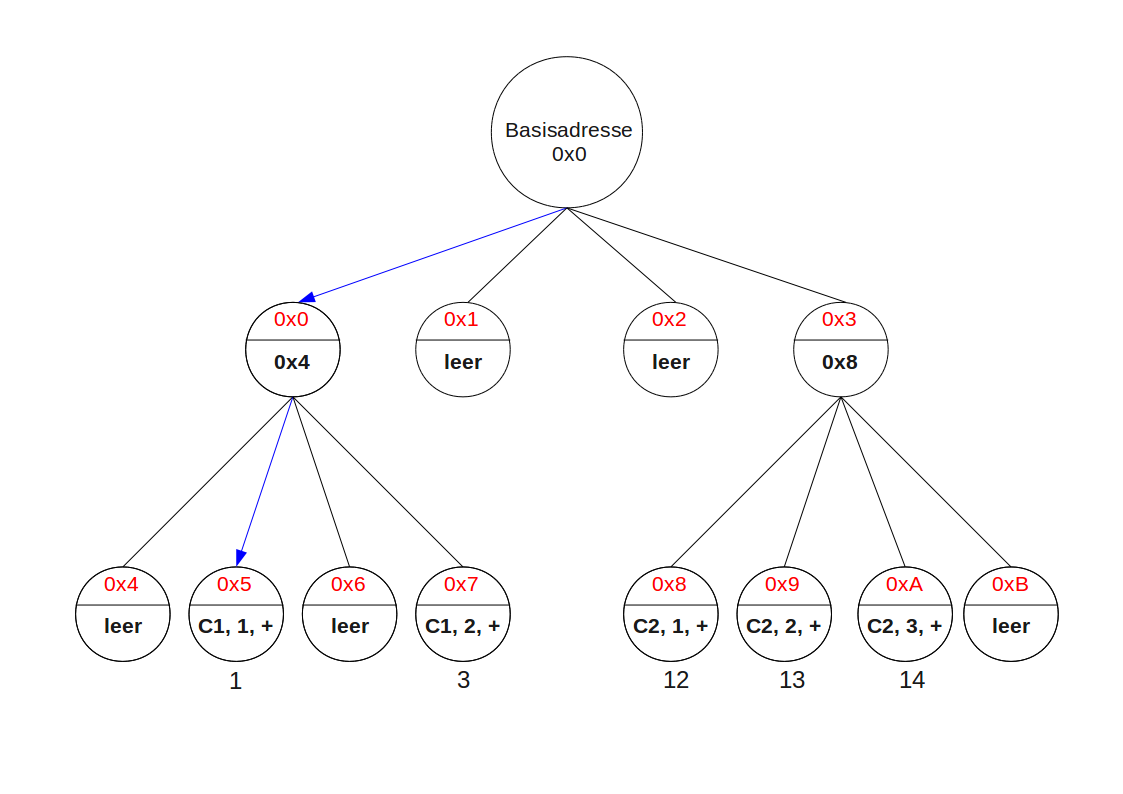
\includegraphics[width=\textwidth]{abb/tree.png}
  \caption{Baumstrukturierter Literal-Lookup}
  \label{tree}
\end{figure}
Mit einem Pfeil ist die Suche nach dem zugehörigen Tupel von 
Variable 1 markiert. Die Binärdarstellung von 1 ist 0001. Geteilt
in zwei Teile ergibt sich $t_1 = 00$ und $t_2 = 01$. Die Basisadresse 0x0 mit dem ersten
Teil $t_1$ addiert 0x0 + 00 ergibt 0x0. An Adresse 0x0 befindet sich die neue
Basisadresse 0x4. Nun addiert man den zweiten Teil $t_2$ mit der neuen Basisadresse
0x4 + 01 was 0x5 ergibt. An Adresse 0x5 findet man nun die Information, dass die Variable positiv ist und 
sich in der ersten Klausel C1 an der ersten Position befindet.\\
Zählt man nun die Knoten des Baumes in Abbildung \ref{tree}, stellt man fest, dass man 12 Knoten 
braucht, um diesen Baum aufzubauen. In Tabelle \ref{tree_table} ist der
Baum aus Abbildung \ref{tree} im Speicher eines Block-RAMs dargestellt.
\begin{table}[h]
  \centering
  \begin{tabular}{|l|l|l|}
    \hline
    \textsc{Speicheradresse} & \textsc{Daten}\\
    \hline
    0x0 & 0x4\\
    \hline
    0x1 & leer\\
    \hline
    0x2 & leer\\
    \hline
    0x3 & 0x8\\
    \hline
    0x4 & leer\\
    \hline
    0x5 & C1, 1, +\\
    \hline
    0x6 & leer\\
    \hline
    0x7 & C1, 2, +\\
    \hline
    0x8 & C2, 1, +\\
    \hline
    0x9 & C2, 2, +\\
    \hline
    0xA & C2, 3, +\\
    \hline
    0xB & leer\\
    \hline
    ... & ...\\
    \hline
  \end{tabular}
  \caption{Darstellung des Baumes aus Abbildung \ref{tree} im Speicher}
  \label{tree_table}
\end{table}
Man könnte sogar noch weitere Variablen 
hinzufügen, ohne weitere Knoten anlegen zu müssen (Wertetupel von 2 und 15).
Man kann also mit diesem Baum 8 von 15 Variablen referenzieren.
Allerdings kann man diese 8 Variablen nicht beliebig wählen.
Würde man zum Beispiel versuchen, Variable 4 in den Baum einzufügen müsste man 
den Knoten mit Adresse 0x1 expandieren, was eine Belegung von 4 weiteren 
Speicherplätzen mit sich führt.\\
Das Gruppieren von Formeln muss für diesen baumstruckturierten Literal-Lookup
weitere Bedingungen erfüllen. Hierfür werden folgende Begriffe eingeführt.

\begin{definition}
  Ein Baum $T$ ist ein Baum mit den folgenden Eigenschaften.
  \begin{itemize}
    \item Blätter sind entweder Tupel der Form (CID, POS, POL) oder leer
    \item Jeder nicht Blattknoten hat $2^m$ Kindsknoten und beinhaltet\\
      eine Basisadresse
    \item Die maximale Tiefe des Baumes ist $k/m$
  \end{itemize}
\end{definition}

\begin{function}
  Eine Funktion $tree(G)$ bildet einen Baum $T$ der Gruppe $G$.
\end{function}
\begin{function}
  Eine Funktion $mem(T)$ zählt die Knoten des Baumes $T$
\end{function}
mem(T) ermittelt somit den verbrauchten Speicherplatz. Mit $M$ wird
der verfügbare Speicherplatz bezeichnet.
\begin{function}
  Eine Funktion $add(v, T)$ fügt die Variable $v$ dem Baum $T$ hinzu.
\end{function}
\begin{function}
  Eine Funktion $add(C, T)$ fügt alle Literale $l_i \in C$
  dem Baum $T$ hinzu, indem iterativ die entsprechenden Variablen $v_i = var(l_i)$
  mit $add(v_i, T)$ dem Baum hinzugefügt werden.
\end{function}
Zu den Eigenschaften der Funktion $group: {\cal C} \rightarrow {\cal G}^{(1)}$
kommt nun noch eine weitere Bedingung, ob eine Klausel $C$ einer Gruppe $G_k \in {\cal G}^{(1)}$
hinzugefügt werden kann. Sollte die Relation $mem(add(C, tree(G_k))) \leq M$ erfüllt sein,
dann kann $C$ der Gruppe $G_k$ hinzugefügt werden.
Der Nachteil dieser vorgestellten Technik ist, dass sich der vorhandene Speicher 
für die Variablentupel mit einem Baum geteilt werden muss. Der geteilte Speicher hat zur
Folge, dass weniger Klauseln pro Gruppe möglich sind und somit
auch die Gesamtzahl der möglichen Klauseln sinkt. Es ist jedoch
auch möglich mehr Block-RAM für den Literal-Lookup zur Verfügung
zu stellen. Dann würde sich die Gesamtzahl möglicher Klauseln
nicht vermindern. Mehr Block-Ram ist auf größeren FPGAs
vorhanden, wie sie zum Beispiel von Davis \cite{davis:2008} benutzt werden.
Die Suche nach einem Variabletupel im Baum benötigt mehr Takte
als ein einfacher Speicherzugriff in der Literal-Lookup-Tabelle.
Da der Baum maximal $k/m$ Knoten tief ist, werden 
$k/m$ mal so viele Takte benötigt um ein Wertetupel zu finden.\\
Vorstellbar ist ein Baum mit k = 16 und m = 4. So könnte man 
Probleme mit $2^{16}$ Variablen lösen.

\subsection{Verbesserte Kommunikation zwischen FPGA und \\Host-PC}
\label{kommu}
Eine weitere Möglichkeit die Laufzeit des FPGA-Solvers zu
verbessern, ist es die Kommunikationzeit zwischen
Host-PC und FPGA zu minimieren. Eine Ethernetschnittstelle
ist zwar relativ einfach in Hardware zu implementieren,
jedoch hat sie höhere Latenzen als andere Kommunukationsschnittstellen wie
PCI Express \cite{pcie:2006} oder Hyper-Transport \cite{ht:2006}.
In einem Vergleich \cite{htvspcie:2006} der Latenzen von PCI-E und HT
wurden Übertragungszeiten der beiden Schnittstellen gemessen.
Die Zeiten liegen weit unter der Latenz eines Ethernet-Pakets (300 $\mu$s)
bei ca. 1 $\mu$s.\\
An einigen Stellen im Entwurf ist es nicht unbedingt notwendig,
dass der FPGA auf Antwortpakete des Host-PCs wartet. Angenommen
der FPGA speichert sich die Information ob ein Literal ein Entscheidungsliteral
ist. Im Konfliktfall informiert der FPGA zwar den Host
über die aktuelle Situation, kann dann jedoch den Konflikt
selbst auflösen. Dies würde eine Verschränkung der Kommunikation
zwischen FPGA und Host-PC bedeuten und Kommunikationszeit
einsparen.


\subsection{Conflict Driven Clause Learning Algorithmus}
\label{cdcl}
In diesem Abschnitt soll die Verwendung von CDCL als
Suchalgorithmus zum Lösen von  SAT-Problemen untersucht werden.
Der Conflict Driven Clause Learning Algorithmus (CDCL) ist eine
Erweiterung des \\DPLL-Algorithmus und wurde in \cite{paper:silva:1997} eingeführt.
Der CDCL-Algorithmus versucht aus Konflikten zu lernen. Bei einem Konflikt wird die
entsprechende Konfliktklausel (unerfüllte Klausel, welche einen Konflikt auslöst)
analysiert, eine neue Klausel gelernt und ein Rücksprung über
mehrere Entscheidungsliterale hinweg duchgeführt.\\
Den massiven Geschwindigkeitsgewinn, gegenüber DPLL-Solvern,  
hat ein CDCL-Solver einer vielzahl von eingesetzten Techniken 
zu verdanken.
In der Arbeit von Katebi \cite{katebi:2011} wird untersucht,
welchen Einfluss einzelne Techniken auf das Zeitverhalten
von SAT-Solvern haben. Dabei werden sowohl DPLL- als auch 
CDCL-Solver betrachtet. Folgende Techniken wurden untersucht:\\
\begin{itemize}
\item 
  Two Literal Watching (2WL) \cite{moskewicz:2001}
\item 
  Phase Saving (PHS) \cite{pipatsrisawar:2007}
\item 
  Random Restarts (RST) \cite{gomes:1998}
\item 
  Variable State Independent Decaying Sum (VSIDS) \cite{moskewicz:2001}
\item 
  Clause Learning (CL) \cite{paper:silva:1997}
\end{itemize}
\begin{figure}[h]
  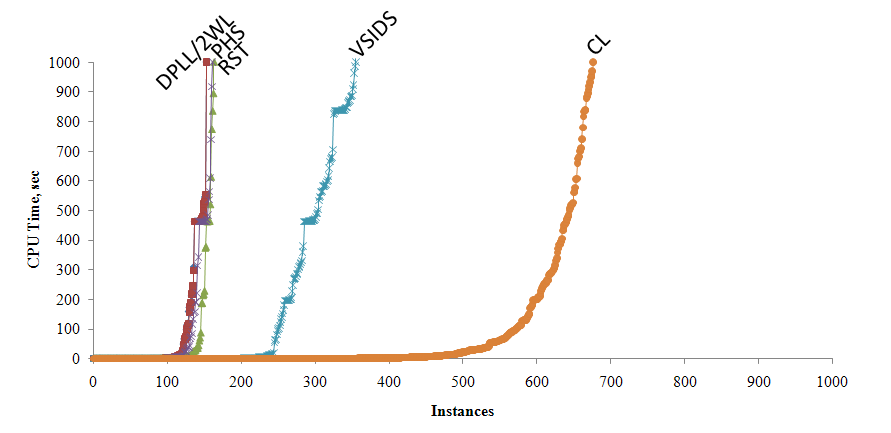
\includegraphics[width=\textwidth]{abb/dpll-teq.png}
  \caption{DPLL-Techniken  \cite{katebi:2011}}
  \label{dpll-teq}
\end{figure}
In Abbildung \ref{dpll-teq} sind die Ergebnisse der Untersuchungen von Katebi, über 1000 SAT-Instanzen,
dargestellt. Beim lösen der Instanzen gibt es ein Zeitlimit von 1000 Sekunden. Man sieht wieviele Instanzen 
der DPLL-Solver durch hinzunahme verschiedener
Techniken lösen kann. Die wenigsten Instanzen löst der reine DPLL-Solver. Auch 
das Erweitern des Solvers durch 2WL, PHS, oder RST ermöglicht es nicht wesentlich
mehr Instanzen zu lösen. Die Techniken VSIDS und CL sorgen für einen starken
Leistungsschub. Wobei sich VSIDS leicht auf dem Host-PC des FPGA-Solvers implementieren
lässt, da es sich um eine Entscheidungsheuristik handelt. Der FPGA müsste dem Host-PC
nur noch die Konfliktklausel mitteilen, da diese für die Berechnung des nächsten
Entscheidungsliterals eine wichtige Rolle spielt. Um CL ohne weiteres implementieren
zu können, müsste es dem FPGA-Solver möglich sein weitere Klauseln zu lernen und
somit seine Klauseldatenbank zu aktualisieren.
Das lernen von Klausel ist jedoch im aktuellen Entwurf nicht vorgesehen. Im
Entwurf von Davis wird eine Technik beschrieben, so dass auch ein FPGA-Solver
Klauseln lernen kann.\\
Abbildung \ref{cdcl-teq} zeigt zusätzlich noch Ergebnisse eines CDCL-Solvers. Es wurden die gleichen 
Instanzen gelöst wie auch in Abbildung \ref{dpll-teq}. Der genutzte CDCL-Solver implementiert alle
oben aufgeführten Techniken. Der Graph, welcher mit $\neg$ CL
beschriftet ist, zeigt die Ergebnisse eines CDCL-Solvers ohne
Clause Learning.
\begin{figure}[h]
  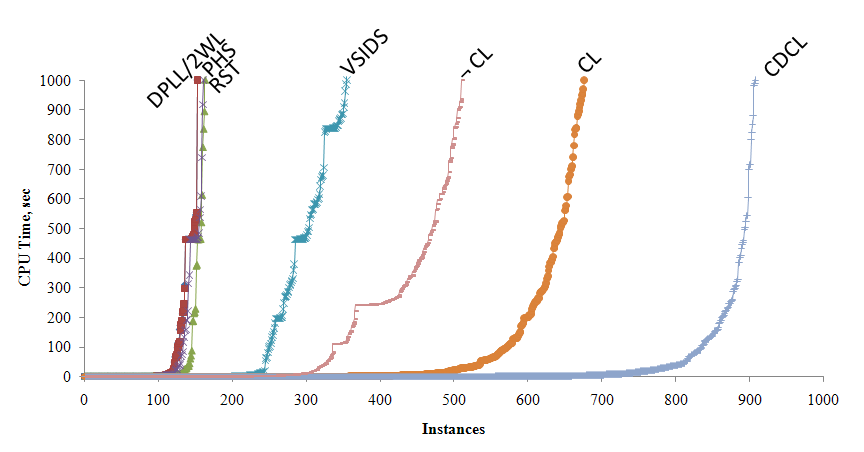
\includegraphics[width=\textwidth]{abb/cdcl-teq.png}
  \caption{CDCL-Techniken \cite{katebi:2011}}
  \label{cdcl-teq}
\end{figure}
Man sieht, das ein CDCL-Solver ohne CL mehr Instanzen löst als
ein DPLL-Solver erweitert mit VSIDS. Es ist also möglich den Algorithmus
des Host-PCs auf CDCL ohne CL umzustellen ohne große Veränderungen
am Entwurf des FPGAs vorzunehmen und trotzdem einen
Leistungsgewinn zu erhalten.


